% !TeX root = ../tfg.tex
% !TeX encoding = utf8
%
% ====================================================================
%  CAPÍTULO 1 — INTRODUCCIÓN DE LA EMPRESA Y ORGANIGRAMA
%
%  RECORDATORIO AL EQUIPO:
%  Este capítulo sitúa al lector. Debe incluir:
%    - Descripción breve pero completa: sector, tamaño, historia reciente,
%      presencia geográfica, número de empleados, cifras clave.
%    - El organigrama: niveles jerárquicos, áreas funcionales y, si es
%      posible, el departamento de RRHH destacado.
%    - Cómo está estructurada la empresa formalmente vs. cómo funciona
%      realmente (funcional, divisional o matricial).
%    - Si tenéis el organigrama como imagen, guardadla en /img/
%      y usad \includegraphics. Si no, describidlo en texto.
%  Fuentes útiles: Memoria Anual CaixaBank, CNMV, web corporativa.
% ====================================================================

\chapter{La empresa: CaixaBank}

% ============================================================
\section{Descripción general}
% ============================================================

% TODO: Ampliad con datos reales obtenidos de la entrevista y fuentes
% oficiales (Memoria Anual CaixaBank, CNMV, web corporativa).
% Actualizad las cifras si han variado desde las que figuran aquí.

CaixaBank, S.A. es una entidad bancaria española con sede central en Valencia.
Surgida de la reorganización del Grupo ``la Caixa'', cotiza en el IBEX~35
y es actualmente uno de los mayores grupos financieros de España y Portugal
tras la fusión con Bankia completada en 2021.

\begin{table}[H]
  \centering
  \caption{Datos corporativos básicos de CaixaBank}
  \begin{tabularx}{\textwidth}{lX}
    \toprule
    \textbf{Parámetro}           & \textbf{Valor} \\
    \midrule
    Sector                       & Servicios financieros y bancarios \\
    Año de fundación             & 1904 (origen en Caja de Pensiones para la Vejez y de Ahorros) \\
    Sede central                 & Valencia, España \\
    Número de empleados          & $\sim$45.000 (grupo consolidado, 2024) \\
    Número de oficinas           & $\sim$4.000 en España \\
    Presencia internacional      & Portugal (BPI), Luxemburgo, Reino Unido, entre otros \\
    Cotización                   & IBEX~35 (ticker: CABK) \\
    Facturación / Margen bruto   & \mejora{Margen bruto de intereses: $\sim$10.100 millones de euros (2024)} \\
    \bottomrule
  \end{tabularx}
\end{table}

\begin{sidewaysfigure}[p]
  \centering
  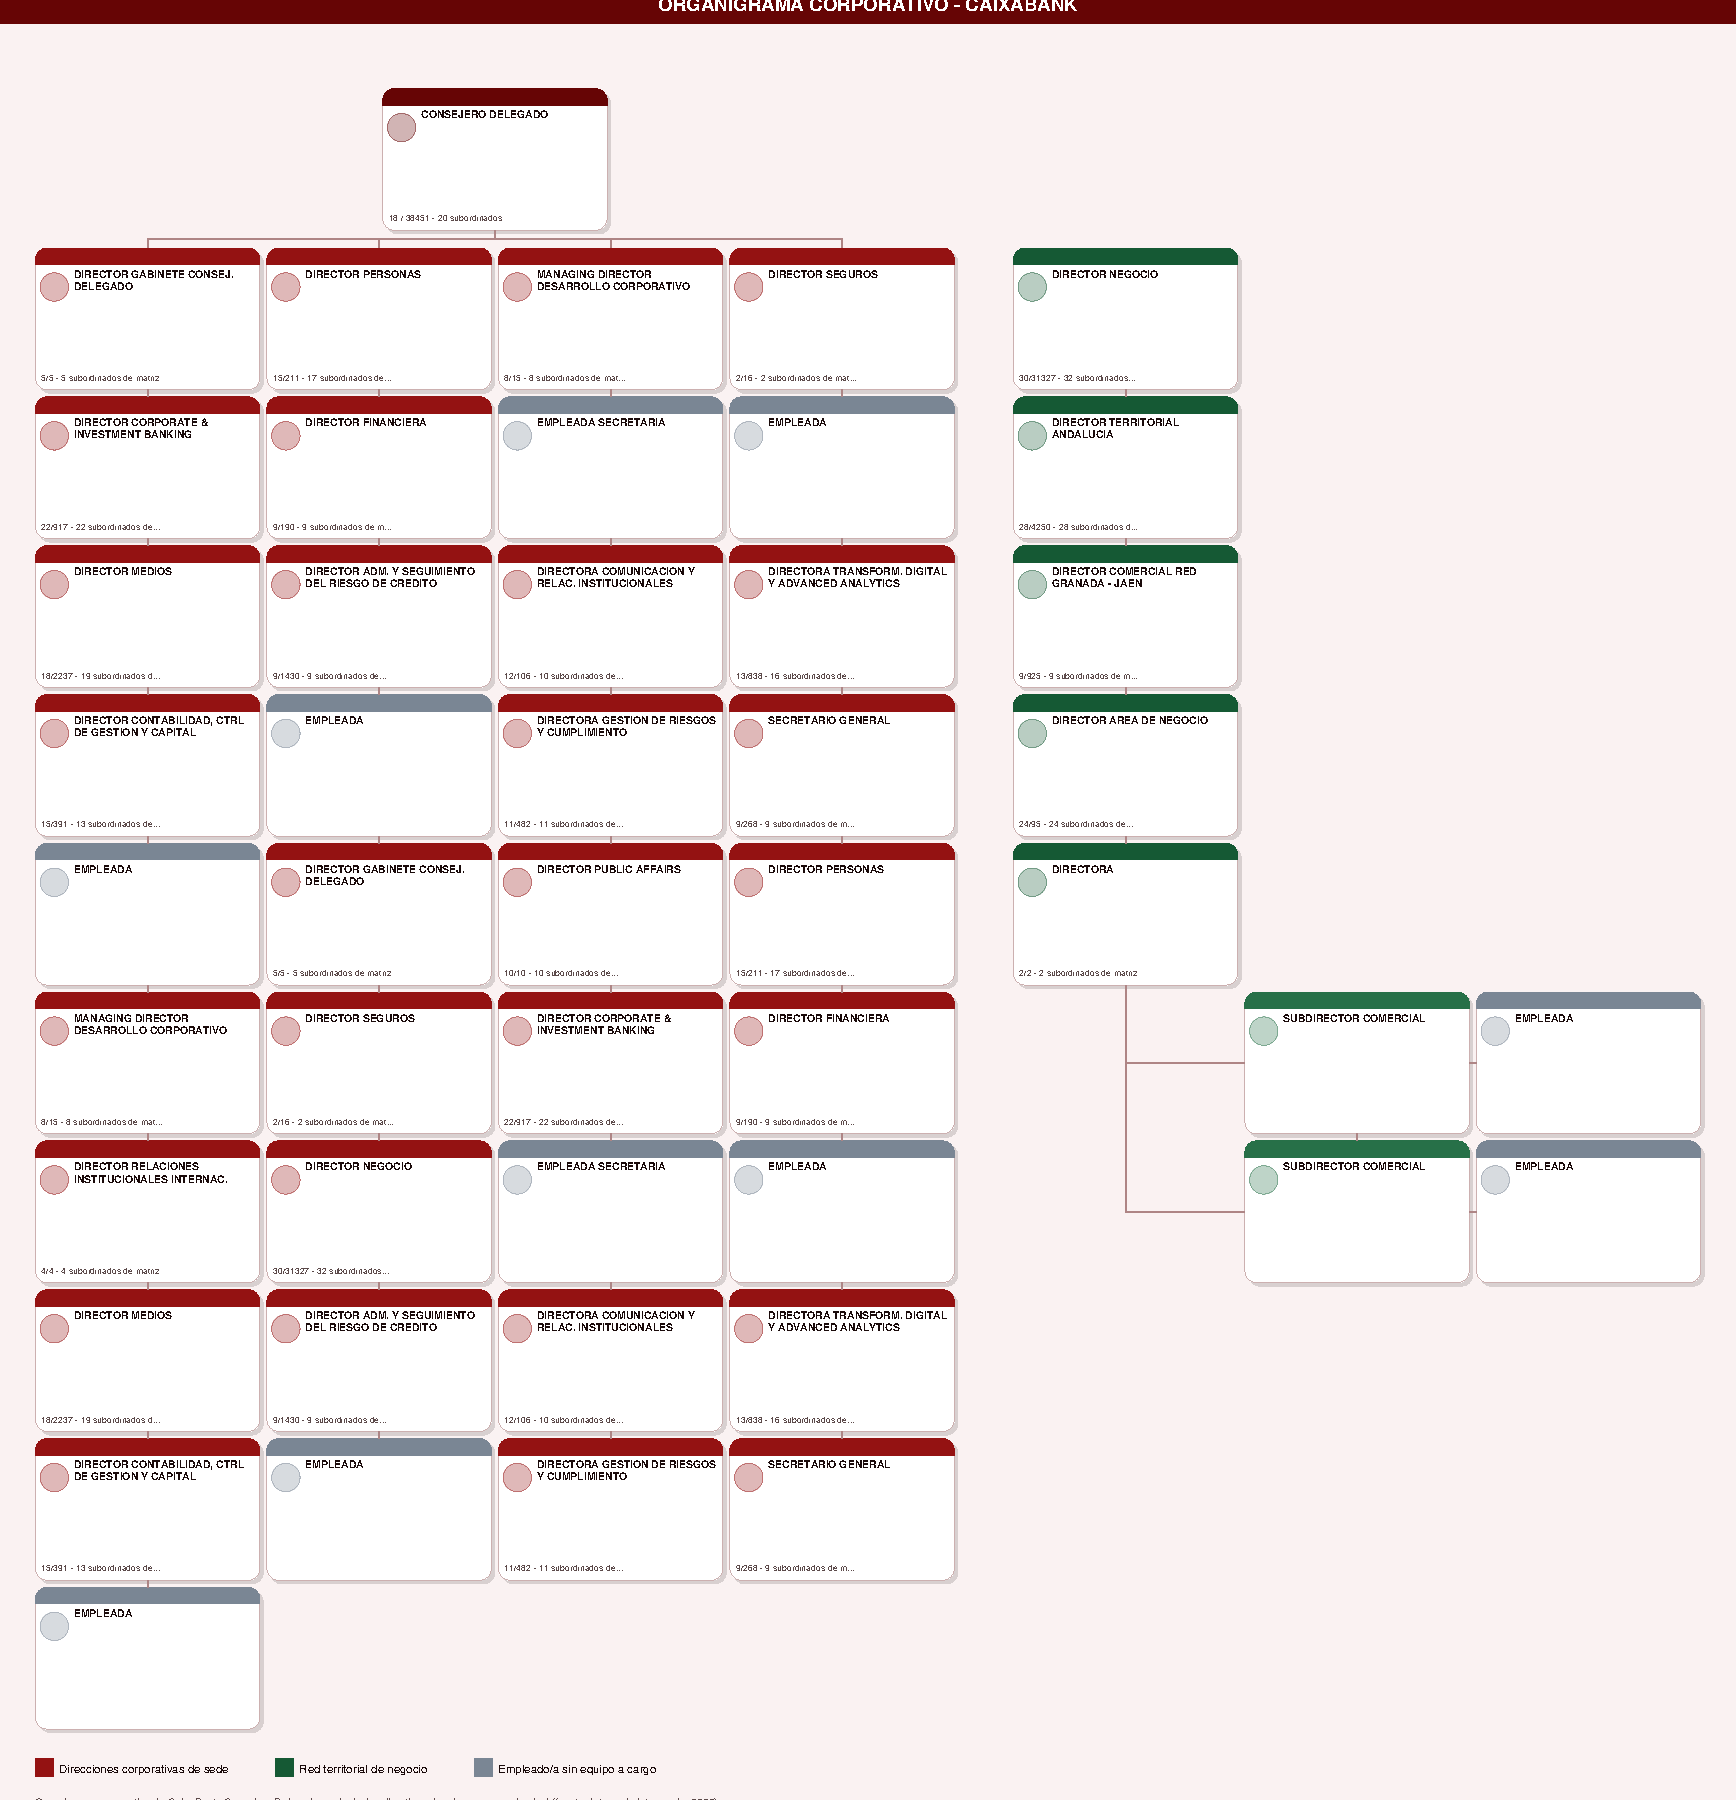
\includegraphics[height=0.8\textwidth,width=0.8\textheight,keepaspectratio]{organigrama}
  \caption{Organigrama corporativo de CaixaBank: Consejero Delegado y principales directivos de primer y segundo nivel (fuente: Interna\,/\,elaboraci\'on propia, 2026).}
\label{fig:organigrama}
\end{sidewaysfigure}

% ============================================================
\section{El departamento de Personas y Organización (RRHH)}
% ============================================================

\begin{bloquedemejora}
El departamento responsable de la gestión del capital humano en CaixaBank recibe
el nombre de \textbf{Área de Personas y Organización}. Su misión es atraer,
desarrollar y retener el talento necesario para garantizar la competitividad
del grupo bancario en un contexto de intensa transformación digital.

\medskip
\textbf{Estructura y modelo de funcionamiento.}
El Área de Personas y Organización se articula en torno a dos grandes pilares:
\begin{itemize}
  \item \textbf{Centros de Excelencia (CoE):} Equipos especializados en áreas
        como adquisición de talento (\textit{Talent Acquisition}), desarrollo
        del liderazgo, compensación y beneficios, relaciones laborales y
        People Analytics.
  \item \textbf{\textit{Business Partners} de RRHH:} Profesionales de Personas
        asignados a cada dirección territorial o área de negocio, actuando como
        puente entre las necesidades locales y las políticas corporativas.
\end{itemize}
\end{bloquedemejora}

\begin{table}[H]
  \centering
  \small
  \caption{\mejora{Áreas funcionales del departamento de Personas y Organización de CaixaBank}}
  \begin{tabularx}{\textwidth}{p{0.38\textwidth} X}
    \toprule
    \textbf{Área}                       & \textbf{Responsabilidades principales} \\
    \midrule
    Talent Acquisition                  & Reclutamiento interno y externo, employer branding, programas de talento joven. \\
    People Development                  & Gestión de carrera, planes de sucesión, coaching, mentoring y assessment. \\
    Learning \& Development             & Diseño y gestión de la plataforma Evoluciona, formación normativa y certificaciones externas. \\
    People Analytics                    & Explotación del SIRH (SAP SuccessFactors), KPIs de capital humano, informes para el comité de dirección. \\
    Compensación y Beneficios           & Estructura salarial, retribución flexible, benchmarking retributivo y administración del convenio colectivo. \\
    Relaciones Laborales                & Negociación sindical, gestión de EREs y conflictos colectivos, cumplimiento normativo laboral. \\
    Secretaría Técnica de Negocios      & Análisis y definición de puestos en colaboración con consultoras externas (Deloitte). \\
    \bottomrule
  \end{tabularx}
\end{table}
